\section{电池}\label{sec:7-5}

\begin{wrapfigure}[12]{r}{7cm}
    \centering
    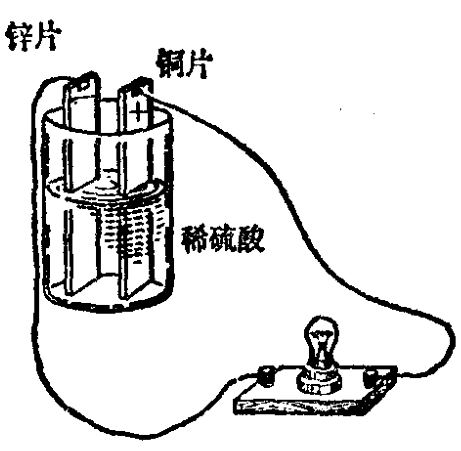
\includegraphics[width=6cm]{../pic/czwl2-ch7-10}
    \caption{用伏打电池给小灯泡供电}\label{fig:7-10}
\end{wrapfigure}

电池是日常生活中和实验室里常用的电源。
最初的电池是十九世纪初意大利物理学家伏打发明的,叫伏打电池。
把一块铜片和一块锌片,浸在稀硫酸溶液里,就做成了一个伏打电池,
它可以向小灯泡供电,使小灯泡发光(图 \ref{fig:7-10})。
在伏打电池里,由于发生了化学变化,在铜片上聚集了正电荷,在锌片上聚集了负电荷。
铜片和锌片叫做伏打电池的电极。
聚集正电荷的铜片叫\textbf{正极},
聚集负电荷的锌片叫\textbf{负极}。
用导线把小灯泡连接到电池的两极间时,电流从电池的正极流出,经过导线和小灯泡,流回电池的负极。
所以,\CJKunderwave{导线中电流的方向是从电池的正极流向负极}。

用伏打电池作电源,小灯泡很快就暗下来,表明通过灯丝的电流迅速地减弱。
所以这种电池实用价值不大,现在最常用的电池是干电池。

干电池的外壳是一个锌筒,\CJKunderwave{锌筒是干电池的负极},也是干电池的容器,里面装着化学药品。
锌筒中央的\CJKunderwave{碳棒是干电池的正极}(图 \ref{fig:7-11})。

\begin{figure}[htbp]
    \centering
    \begin{minipage}{7cm}
    \centering
    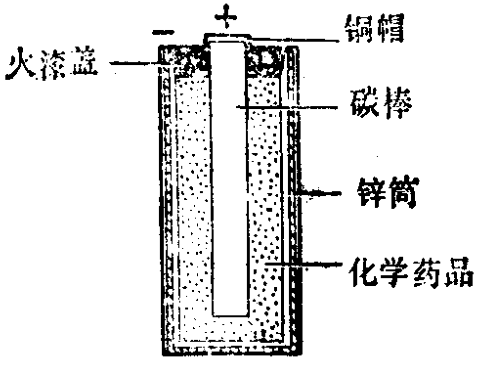
\includegraphics[width=6cm]{../pic/czwl2-ch7-11}
    \caption{干电池剖面图}\label{fig:7-11}
    \end{minipage}
    \qquad
    \begin{minipage}{7cm}
    \centering
    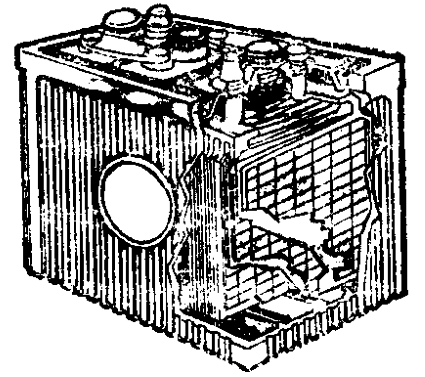
\includegraphics[width=6cm]{../pic/czwl2-ch7-12}
    \caption{铅蓄电池}\label{fig:7-12}
    \end{minipage}
\end{figure}


干电池连续使用长了电流会减弱,所以干电池适合于断续的工作,
半导体收音机、手电筒等等常用干电池作电源。

干电池用过相当长的时间以后,就不能再用了,必须换新的。
这类电池叫一次电池,也叫原电池。
还有一类电池叫蓄电池,可以多次充电重复使用。

图 \ref{fig:7-12} 是常用的铅蓄电池。这种电池是把许多块铅板放在稀硫酸里做成的。
铅板分为两组,一组是正极,一组是负极,它们的接线柱上分别有 “$+$” 、“$-$” 的标记。

为了使蓄电池能向外供电,需要先给它充电。
充电的时候,要把蓄电池的正、负极分别接到另一个电源的正、负极上,电流通过蓄电池,
使蓄电池内部发生化学变化,电能转化为化学能,储蓄在蓄电池里。
蓄电池向外供电叫做放电,放电的时候,它储蓄的化学能又转化为电能。

蓄电池的应用很广。汽油机的点火,汽车、火车、飞机的照明,等等,都要用到蓄电池。
做物理实验的时候也常常用蓄电池作为电源。

使用蓄电池的时候,\CJKunderwave{绝对不允许用导线直接把两极连接起来}(其他电源也不允许这样做),
因为那样放电电流太大,会损坏蓄电池。蓄电池用过一段时间以后,需要及时给它充电,不然也会损坏。

上面讲到的几种电池,都是利用化学变化来供电的。
从能量转化的观点来看,它们的作用都是把化学能转化成电能。这样的电池又叫做化学电池。


\section*{阅读材料:新型电池}

干电池、铅蓄电池的应用已经有一百多年的历史,它们的性能虽然不断提高,
但是满足不了科学技术各方面飞速发展的需要。因此,近年来新型电池不断出现。

氧化银电池(也叫银锌电池)是一种重量轻而容量\footnotemark 大的新电池,大量用在电子手表、导弹和人造卫星上。
它的负极是锌,正极是氧化银。图 \ref{fig:7-13} 是用于电子手表里的钮扣式微型氧化银电池,可以连续使用一年。
\footnotetext{电池放电电荷的总量叫做电池的容量。}

\begin{figure}[htbp]
    \centering
    \begin{minipage}{8cm}
    \centering
    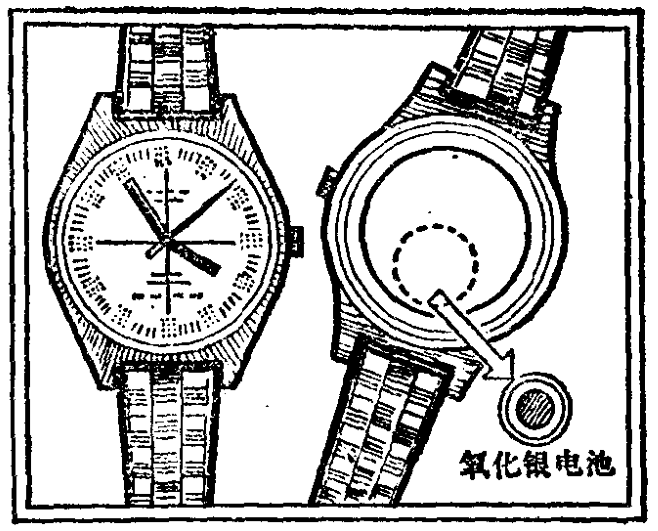
\includegraphics[width=7cm]{../pic/czwl2-ch7-13}
    \caption{电子手表里的微型氧化银电池}\label{fig:7-13}
    \end{minipage}
    \qquad
    \begin{minipage}{6cm}
    \centering
    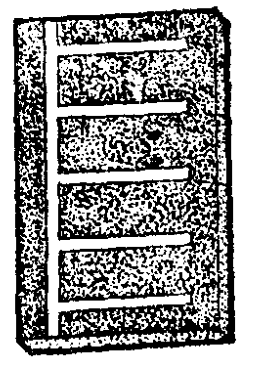
\includegraphics[width=3cm]{../pic/czwl2-ch7-14}
    \caption{硅光电池}\label{fig:7-14}
    \end{minipage}
\end{figure}


锂电池是一种正处于试用阶段尚未大量生产的新型电池,它的负极是锂做的。
这种电池的突出优点是使用寿命长,能在较大的温度范围内工作。

还有一些不属于化学电池的新型电池,例如硅光电池(图 \ref{fig:7-14})。
硅光电池是用硅做成的、把光能转化为电能的电池。
这种电池性能稳定,寿命很长,但目前成本高、价格贵,主要用在人地球卫星上,%(\hyperref[fig:pic4]{彩图4}),
作为卫星携带的实验仪器、通讯设备的电源。
现在,把原子能直接转化为电能的原子电池,也在开始研究试制了。

